\documentclass{jsarticle}
\usepackage{moreverb}
\usepackage[dvipdfmx]{graphicx}
\usepackage{float}

\title{計算機実習 問題12.1 離散的な時間の1次元ランダムウォーク}
\author{早稲田大学先進理工学部物理学科 B4 藤本將太郎}
\date{2014/05/28}

\begin{document}
\maketitle
    
    \section{シミュレーションの目的}
        本シミュレーションでは、ランダムウォークの最も簡単な場合として、並進対称な1次元の格子上を一定の時間間隔で遷移するモデルを考える。ランダムウォークの分散について知られていることとして、十分大きな$N$に対して$< \Delta x^{2}(N)> $はべき乗則
        \begin{equation}
            <\Delta x^{2}(N)> \sim N^{2\nu}
            \label{eq:e1}
        \end{equation}
        を満たす。ここで記号$\sim$は"漸近的に等しい"ことを意味し、式(\ref{eq:e1})は漸近的なスケーリング則の1例となっている。今簡単な1次元ランダムウォークのモデル(右と左に進む確率が等しいとき)では、すべての$N$で式(\ref{eq:e1})が成り立ち、$\nu = 1/2$ となる。

    \section{作成したプログラム}
        本シミュレーションで作成したプログラムを以下に示す。
    
    
        \subsection{1次元ランダムウォークのシミュレーション(12-1\_random\_walk\_d1.py)}
        このプログラムでは、右に遷移する確率をprobとして指定し、numpyモジュールの乱数生成メソッドを用いて、ランダムな[0,1)の数を配列pに格納している。各ステップごとにprobの値と乱数の値とを比較して、右か左にlだけ変化させた値を次の時間での変位として記録する(今はl=1)。関数calc\_aveでは、$<x(N)> $、$< x^{2}(N)> $の値を計算する。関数showを用いると、上の計算結果をもちいて、$N$に対する$<x(N)> $、$<x^{2}(N)> $、$<\Delta x^{2}(N)> $のグラフを表示することができる。関数caluculate\_errorは問題bで使用し、引数に与えた整数値までのランダムウォークの計算を行って、試行回数を増やしていったときに$< \Delta x^{2}(N)> $の精度が1%未満になっているかどうかを判定する。
            \listinginput{1}{12-1_random_walk_d1.py}
            
    \section{実習課題}
    
        \begin{enumerate}
            \renewcommand{\labelenumi}{\alph{enumi}.}
            \renewcommand{\labelenumii}{}
            
            \item 右に動く確率を$p=0.7$とする。$< x(N)> $と$< x^{2}(N)> $を$N=4,8,16,32$について計算せよ。この場合の$< x(N)> $はどのように説明できるか。$< \Delta x^{2}(N)> $がどう$N$に依存するか定性的に答えよ。$< x^{2}(N)> $は単純な$N$依存性を示すか。
                
                \begin{enumerate}
                    \item $< x(N)> $と$< x^{2}(N)> $、$< \Delta x^{2}(N)> $について、$\mathrm{nwalkers}=1000$としてそれぞれの$N$について計算を行い、この結果を横軸を$N$としてグラフにしたものを図\ref{fig:f1}に示す。このグラフから読み取れることとして、まず、$< x(N)> $は$N$に対して線形に増加しており、これは以下のような簡単な計算の結果と一致している。また、傾きの大きさも$2p-1=0.4$となっていることが分かる。
                    \begin{eqnarray}
                        <x(N)>  &=& \sum_{i=1}^{N}\{ p\times 1 + (1-p)\times (-1)\} \\
                        &=& \sum_{i=1}^{N}(2p-1) = (2p-1)N
                    \end{eqnarray}
                    次に、$< \Delta x^{2}(N)> $については、$N$の1乗に比例していることが見て取れる(すなわち$\nu = 1/2$である)。これも、一般の場合に$< \Delta x^{2}(N)> =4pql^{2}N$と表せることと合致している。
                    
                    \begin{figure}[H]
                        \begin{center}
                            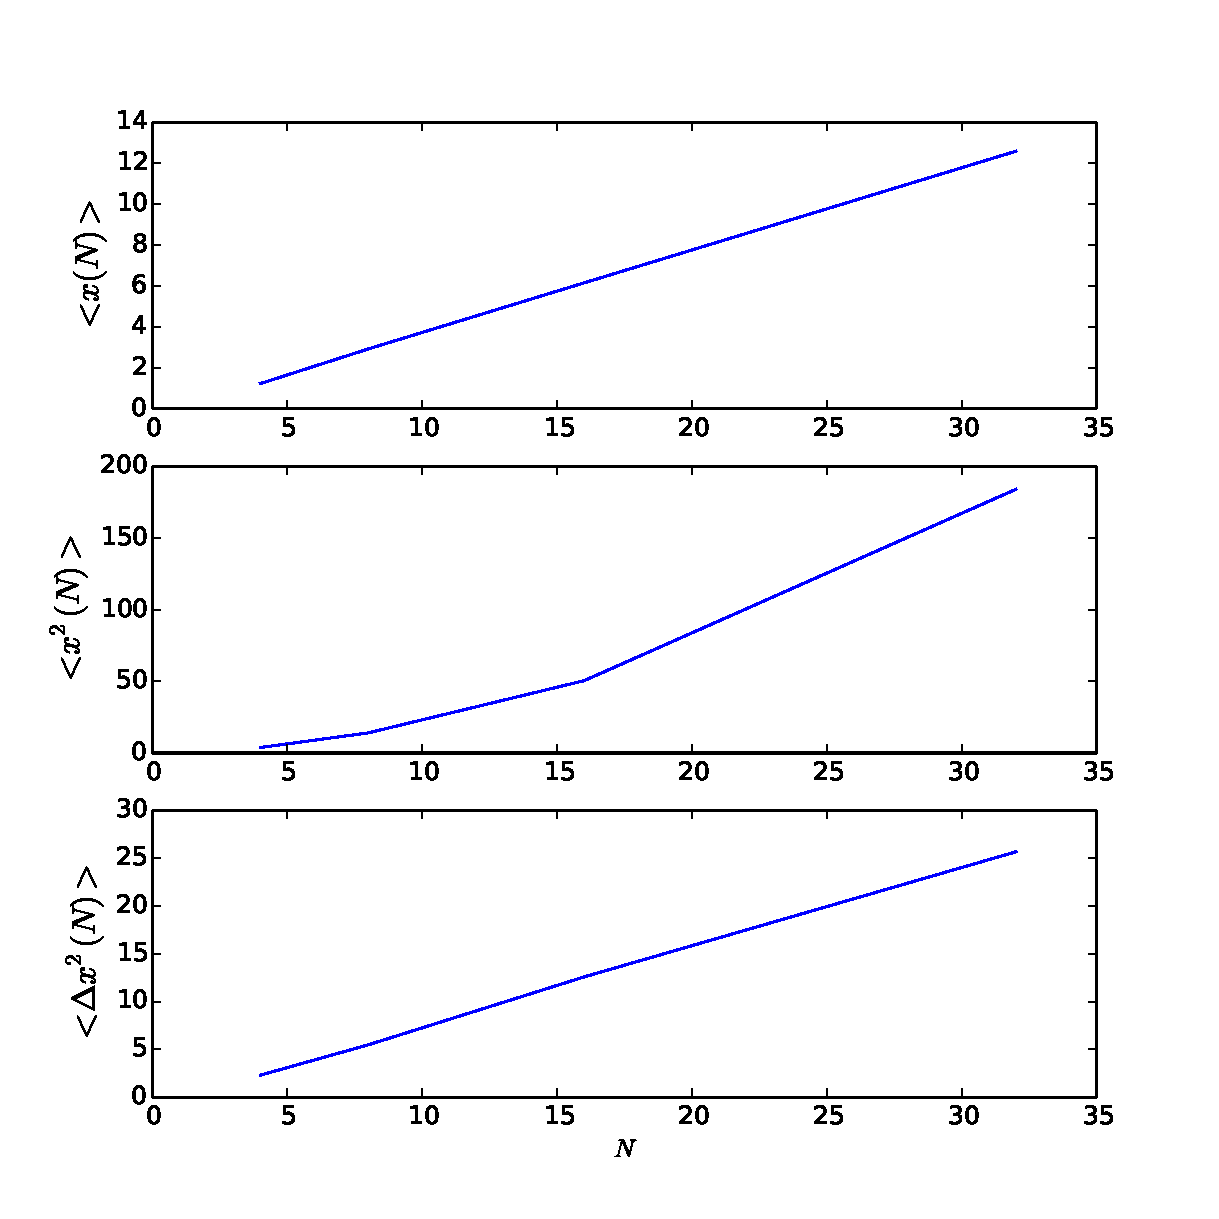
\includegraphics[width=12.5cm]{figure_1.pdf}
                            \caption{$N$に対する$< x(N)> $と$< x^{2}(N)> $、$< \Delta x^{2}(N)> $のグラフ}
                            \label{fig:f1}
                        \end{center}
                    \end{figure}


                \end{enumerate}    
            
            \item 第11.4節で述べた誤差解析の方法を用いて、$N=8$と$N=32$の場合の$< \Delta x^{2}(N)> $を精度1%で得るために必要な試行の回数を求めよ。    
            
                \begin{enumerate}
                    \item (a)で述べたように、解析的に$< \Delta x^{2}(N)> $の値は求められるので、その値を真の値$< \Delta x^{2}(8)> _{0} = 4 \times 0.7 \times 0.3 \times 8 = 6.72$、$< \Delta x^{2}(32)> _{0} = 4 \times 0.7 \times 0.3 \times 32 = 26.88$として、それとの相対誤差が1%となるような試行回数Mを求めればよい。すなわち標準誤差を$\sigma_{m}$として
                    \begin{eqnarray}
                        \frac{\sigma_{m}}{< \Delta x^{2}(N)> _{0}} \times 100 \leq 1 \\
                        \sigma_{m} \leq 0.01 <\Delta x^{2}(N)> 
                    \end{eqnarray}
                    となる。ここで、付録に示すように、$n$回の試行を行う1回の測定で得られた分散を$\sigma$とすると
                    \begin{equation}
                        \sigma_{m} = \frac{\sigma}{\sqrt{n}}
                    \end{equation}
                    が成り立つので、これを代入すると($n$を$M$と読み替えて)
                    \begin{equation}
                        M \geq \left( \frac{\sigma\times 100}{< \Delta x^{2}(N)>_{0}}\right) ^{2}
                        \label{eq:e2}
                    \end{equation}
                    が得られる。$\sigma$が$M$の関数として決まっている場合は、$M$の値を解析的に求めることができるが、今の場合$\sigma$を$M$の関数として求める方法はわからない。したがって、$M$の値を2から順に大きくしていき、$M$の値と式(\ref{eq:e2})の右辺の計算値とを比較していくことにする。この結果をまとめたものを表\ref{t1},\ref{t2}に示す。これらの試行から、$< \Delta x^{2}(N)> $を精度1%で得るために必要な試行の回数$M$は、$\mathrm{nwalkers}=1000$であるときには、$N=8$のとき$M\geq 19$、$N=32$のとき$M\geq 26$ほどであれば良いことが分かる。それより小さい$M$では、精度1%で求められることもあるが、下限値として適切ではない。
                    \begin{table}[H]
                        \begin{center}
                            \begin{tabular}{cc}

                                \begin{minipage}{0.5\hsize}
                                    \begin{center}
                                    \begin{tabular}{rcl|c}
                                        M &     & $\left( \frac{\sigma\times 100}{< \Delta x^{2}(N)>_{0}}\right) ^{2}$ & count \\ \hline
                                        2 & $<$ & 11.7080095291 & \\
                                        3 & $<$ & 10.5683527683 & \\
                                        4 & $<$ & 5.6449783206 & \\
                                        5 & $<$ & 13.1767199401 & \\
                                        6 & $<$ & 9.31017539915 & \\
                                        7 & $<$ & 11.298006385 & \\
                                        8 & $<$ & 11.6122000702 & \\
                                        9 & $<$ & 11.8588271339 & \\
                                        10 & $<$ & 13.2805462695 & \\
                                        11 & $>$ & 5.40663459242 & 1 \\
                                        12 & $>$ & 11.6587313198 & 2 \\
                                        13 & $>$ & 5.20198341922 & 3 \\
                                        14 & $<$ & 14.0913796119 & \\
                                        15 & $>$ & 13.2349559502 & 4 \\
                                        16 & $>$ & 9.20886425624 & 5 \\
                                        17 & $>$ & 10.1345045153 & 6 \\
                                        18 & $<$ & 18.5593052103 & \\
                                        19 & $>$ & 11.0536600843 & 7 \\
                                        20 & $>$ & 11.5386838619 & 8 \\
                                        21 & $>$ & 13.1460283992 & 9 \\
                                        22 & $>$ & 8.39227718357 & 10 \\
                                        23 & $>$ & 15.8071381158 & 11 \\
                                        24 & $>$ & 8.9317879812 & 12 \\
                                        25 & $>$ & 17.2226656569 & 13 \\
                                        26 & $>$ & 12.3538617431 & 14 \\
                                        27 & $>$ & 11.7846823015 & 15 \\ \hline
                                    \end{tabular}
                                    \caption{$N=8$のとき、$M$と式(\ref{eq:e2})の右辺との比較($\mathrm{nwalkers}=1000$)} 
                                    \label{t1}
                                    \end{center}
                                \end{minipage}
                                
                                \begin{minipage}{0.5\hsize}
                                    \begin{center}
                                    \begin{tabular}{rcl|c}
                                        M &     & $\left( \frac{\sigma\times 100}{< \Delta x^{2}(N)>_{0}}\right) ^{2}$ & count \\ \hline
                                        2 & $>$ & 0.32149282727 & 1 \\
                                        3 & $>$ & 1.02405794329 & 2 \\
                                        4 & $<$ & 30.0521604962 & \\
                                        5 & $<$ & 7.13793428824 & \\
                                        6 & $<$ & 17.593509665 & \\
                                        7 & $<$ & 17.952294418 & \\
                                        8 & $>$ & 5.56611217356 & 3 \\
                                        9 & $<$ & 13.868141118 & \\
                                        10 & $<$ & 17.3761782997 & \\
                                        11 & $>$ & 10.5719588472 & 4 \\
                                        12 & $<$ & 17.9530873904 & \\
                                        13 & $<$ & 17.977542833 & \\
                                        14 & $<$ & 21.0129775506 & \\
                                        15 & $<$ & 16.105658749 & \\
                                        16 & $<$ & 17.2696667207 & \\
                                        17 & $<$ & 29.1796778766 & \\
                                        18 & $>$ & 17.1884240052 & 5 \\
                                        19 & $>$ & 14.4165685045 & 6 \\
                                        20 & $>$ & 16.5500505218 & 7 \\
                                        21 & $>$ & 9.49101301793 & 8 \\
                                        22 & $>$ & 10.7188319627 & 9 \\
                                        23 & $<$ & 29.1758785194 & \\
                                        24 & $>$ & 13.1087274658 & 10 \\
                                        25 & $<$ & 26.9290290068 & \\
                                        26 & $>$ & 20.6962324661 & 11 \\
                                        27 & $>$ & 21.9648359983 & 12 \\
                                        28 & $>$ & 20.7435187729 & 13 \\
                                        29 & $>$ & 18.3682158692 & 14 \\
                                        30 & $>$ & 24.8443920402 & 15 \\ \hline
                                    \end{tabular}
                                    \caption{$N=32$のとき、$M$と式(\ref{eq:e2})の右辺との比較($\mathrm{nwalkers}=1000$)}  
                                    \label{t2}
                                    \end{center}
                                \end{minipage}
                                
                            \end{tabular}
                        \end{center}
                    \end{table}
                            
                \end{enumerate} 
            
        \end{enumerate}
    
    \section{まとめ}
        このシミュレーションでは、離散時間の1次元ランダムウォークの簡単な例を実施することができた。また、測定の精度を上げるために試行回数を増やすことなど、定量的な誤差について学ぶ機会となった。
    \section{付録: 平均値の標準偏差}
        $\sigma$を測定の標準偏差とすると、$n$回の試行からなる単独の測定の誤差が$\sigma/\sqrt n$に等しくなることを、解析的に導く。注目する測定量を$x$で表し、それぞれが$n$回の試行からなる$m$組の、合計して$mn$回の試行からなる測定の組を考える。特定の測定を表すために添字$\alpha$を使い、ある測定の$i$回目の試行を表すために添字$i$を用いる。測定$\alpha$の$i$回目の試行の結果を$x_{\alpha, i}$で表すと、測定の値は
        \begin{equation}
            M_{\alpha} = \frac{1}{n}\sum_{\alpha = 1}^{n}x_{\alpha, i}    
        \end{equation}

        で与えられる。さらに$mn$回のすべての試行についての平均$\bar{M}$は
        \begin{equation}            
            \bar{M} = \frac{1}{m}\sum_{\alpha=1}^{m}M_{\alpha} = \frac{1}{mn} \sum_{\alpha}^{m}\sum_{i=1}^{n} x_{\alpha , i}
        \end{equation}
        となる。$\alpha$番目の測定値とすべての測定の平均値との差は
        \begin{equation}           
            e_{\alpha} = M_{\alpha} - \bar{M}
        \end{equation}
        である。平均値の分散は
        \begin{equation}         
        \sigma_{m}^{2} = \frac{1}{m}\sum_{\alpha=1}^{m} e_{\alpha}^{2}
        \label{eq:e3}
        \end{equation}
        と書くことができる。\\
        $\sigma_{m}$と各測定の試行の分散との関係を調べることにしよう。個々の試行結果$x_{\alpha, i}$と平均値との差$d_{\alpha, i}$は
        \begin{equation}       
        d_{\alpha, i} = x_{\alpha, i} - \bar{M}
        \end{equation}
        で与えられる。したがって、$nm$回の試行についての分散$\sigma^{2}$は
        \begin{equation}        
        \sigma^{2} = \frac{1}{mn}\sum_{\alpha = 1}^{m}\sum_{i=1}^{n}d_{\alpha, i}^{2}
        \label{eq:e7}
        \end{equation}
        である。また、
        \begin{eqnarray}
            e_{\alpha} = M_{\alpha} - \bar{M} &=& \frac{1}{n}\sum_{i=1}^{n}(x_{\alpha, i} - \bar{M}) \\
        &=& \frac{1}{n}\sum_{i=1}^{n}d_{\alpha, i}
        \label{eq:e4}
        \end{eqnarray}
        である。したがって、式(\ref{eq:e4})を(\ref{eq:e3})に代入すると、
        \begin{equation}       
        \sigma_{m}^{2} = \frac{1}{m}\sum_{\alpha - 1}^{m}\left( \frac{1}{n}\sum_{i=1}^{n}d_{\alpha, i}\right) \left( \frac{1}{n}\sum_{j = 1}^{n}d_{\alpha, j} \right)
        \label{eq:e5}
        \end{equation}
        が得られる。式(\ref{eq:e5})の組$\alpha$についての試行$i$,$j$に関する和には2種類の項、つまり、$i=j$の項と$i\neq j$の項が含まれている。$d_{\alpha, i}$と$d_{\alpha, j}$は互いに独立で、平均値としては正と負の値を同程度に取ることが予想されるので、測定回数の大きい極限では、式(\ref{eq:e5})で$i=j$の項だけが和に寄与すると考えてよいだろう。したがって、
        \begin{equation}        
            \sigma_{m}^{2} = \frac{1}{mn^{2}}\sum_{\alpha=1}^{m}\sum_{i = 1}^{n}d_{\alpha, i}
            \label{eq:e6}
        \end{equation}
        と書く。式(\ref{eq:e6})と(\ref{eq:e7})を組み合わせると、求めていた式
        \begin{equation}        
        \sigma_{m}^{2} = \frac{\sigma^{2}}{n}
        \end{equation}
        が導かれる。

    \section{追記: $<x^{2}(N)>$の解析的な値 (2014/06/09)}
    問題aでは$N$に対する$<x^{2}(N)>$について図\ref{fig:f1}を用いて定性的に述べたが、これを解析的に求めるとするとどうなるか。確率pで右に移動し、確率qで左に移動する場合を考えると、このとき$x^{2}(N)$は2つの項の和で表すことができて、$x_{0}=0$ならば
        
        \begin{equation}
            x^{2}(N) = \sum_{i=1}^{N}s_{i}^{2} + \sum_{i\neq j=1}^{N}s_{i}s_{j}
        \end{equation}
        
        である。ここで$s_{i} = \pm l$とする。上の式を利用して$x^{2}(N)$の期待値を計算すると、
        \begin{equation}
            <x^{2}(N)> = \sum_{i=1}^{N}\left[ p(+l)^{2}+q(-l)^{2} \right]  + \sum_{i\neq j=1}^{N}\left[ p(+l)+q(-l) \right]^{2}
        \end{equation}
        
        である。右辺第2項の和は、$(i,j)$の組み合わせ(区別できる)から$i=j$の場合の$N$通りを除いた数だけの場合があるので
        \begin{equation}
            <x^{2}(N)> = N(p+q)l^{2} + N(N-1)(p-q)^{2}l^{2}
        \end{equation}
        
        となる。したがって
        \begin{eqnarray*}
            <x^{2}(N)> &=& Nl^{2} + N(N-1)(p-q)^{2}l^{2} \\
            &=& Nl^{2}\left[ (p+q)^{2}-(p-q)^{2} \right] + N^{2}(p-q)^{2}l^{2} \\
            &=& 4pql^{2}N + N^{2}(p-q)^{2}l^{2}
        \end{eqnarray*}

        である。また、これより$<\Delta x^{2}(N)>$は
        \begin{eqnarray*}
            <\Delta x^{2}(N)> &=& <x^{2}(N)>-(<x(N)>)^{2} = 4pql^{2}N + N^{2}(p-q)^{2}l^{2} - N^{2}(p-q)^{2}l^{2} \\
            &=& 4pql^{2}N
        \end{eqnarray*}
        
        と求められる。以上から$<x^{2}(N)>$はNの2乗に比例しており、実際にシミュレーションで行った$\alpha=0.7$、$N=30$のときの値を計算してみると、$<x^{2}(30)>=4\times 0.7 \times 0.3 \times 30 + 30^{2}(0.7-0.3)^{2} = 169.2$であり、図\ref{fig:f1}で見た値と一致していることが確かめられる。

        
    \section{参考文献}
        \begin{itemize}
            \item ハーベイ・ゴールド,ジャン・トボチニク,石川正勝・宮島佐介訳『計算物理学入
            門』,ピアソン・エデュケーション, 2000.
            \item 鈴木武・山田作太郎著『数理統計学―基礎から学ぶデータ解析―』, 内田老鶴圃, 2008.
        \end{itemize}

\end{document}
